\documentclass[a4paper]{article}

% The following packages can be found on http:\\www.ctan.org
\usepackage{graphicx} % for pdf, bitmapped graphics files
%\usepackage{epsfig} % for postscript graphics files
%\usepackage{mathptmx} % assumes new font selection scheme installed
%\usepackage{times} % assumes new font selection scheme installed
\usepackage{amsmath} % assumes amsmath package installed
\usepackage{amssymb}  % assumes amsmath package installed
\usepackage{url}
\usepackage{float}
% \usepackage{cite}
% \usepackage{math}
\usepackage{array}
\usepackage{multirow}

\usepackage{algorithm}
\usepackage{algorithmic}

% \usepackage{times}
% \usepackage{helvet}
\usepackage{courier}

\usepackage[small,bf]{caption}

\usepackage{anysize}
\marginsize{2cm}{2cm}{2cm}{2cm}

\usepackage{color}
\definecolor{darkgreen}{rgb}{0.0,0.5,0.0}
\definecolor{red}{rgb}{1.0,0.0,0.0}

\newcommand{\todo}[1]{ \textcolor{red}{\bf #1}}

\usepackage{algorithm}
\usepackage{algorithmic}
\usepackage[sort&compress]{natbib}

\usepackage[caption=false,font=footnotesize]{subfig}
\usepackage{multirow}
\usepackage{ifpdf}

\begin{document}

\begin{figure}
\vspace{-3.3cm}
\hspace{-2.2cm}
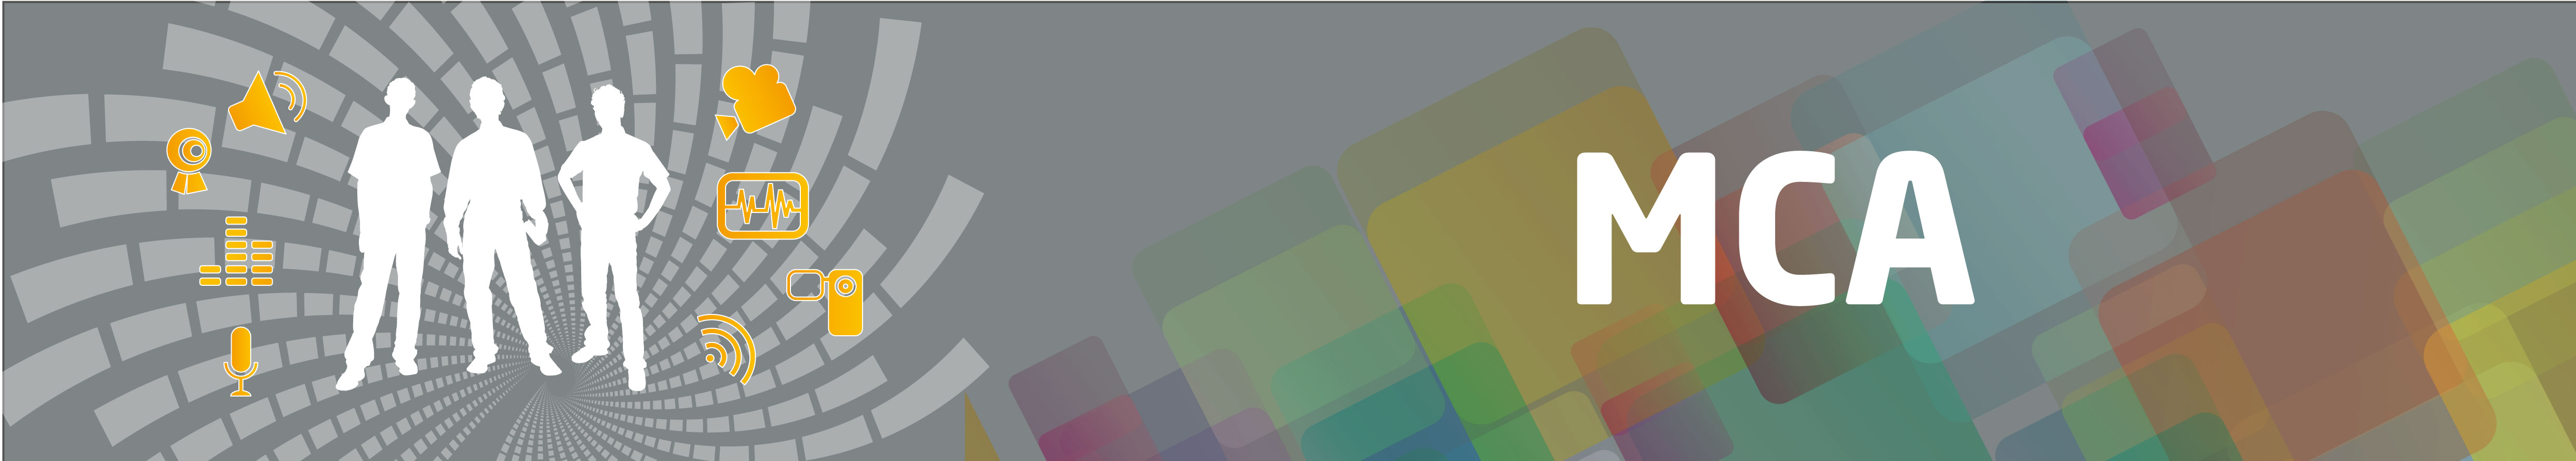
\includegraphics[width=1.25\textwidth]{BannerMCA.jpg}\vspace{0.2cm}\\
\end{figure}


\begin{center}
{\LARGE
Multimodal Conversational Analytics \vspace{0.3cm}\\
\texttt{MCA} Grand Challenge -- Call for papers
} 
\end{center}
\vspace{0.5cm}

\begin{center}
\begin{minipage}{0.92\textwidth}
{\small
The \texttt{MCA} challenge aims to bring together researchers from across disciplines related to multimodal
conversational analytics. The challenge follows the \texttt{D-META} Challenge organized at the ICMI 2012 in Santa
Monica. The \texttt{D-META} challenge had two coupled pillars, method benchmarking and annotation evaluation, and its
starting point was set in transparent and publicly available annotations, tasks, and evaluations on shared multimodal
data sets. This second challenge continues the same tradition.}
\end{minipage}
\end{center}
\vspace{0.5cm}


\begin{center}
\fbox{\begin{minipage}{0.69\textwidth}
Paper dead line: \textbf{15-Jul-2013}.\vspace{0.1cm}\\
Accepted papers will be part of the IEEE/ACM \textbf{ICMI'2013 Proceedings}.
\end{minipage}}
\end{center}

\section*{Scope}
The scope of the \texttt{MCA} challenge concerns the multimodal analysis of primary cues and qualities of conversations.
It proposes to set up the basis for comparison, analysis, and further improvement of multimodal data annotations and
multimodal interactive systems which are important in building various multimodal applications. Such machine
learning-based challenges do not exist in the Multimodal Interaction community, and by focusing on the elaboration of
algorithms and techniques on shared data sets, we aim to foster the research and development of multimodal interactive
systems.\\
The challenge is organized by tasks, which concern three different aspects of multimodal conversational analytics:
\begin{description}
\item[MCA-Engagement] Level of engagement in video-mediated group conversation.
\item[MCA-Gestures] Feedback and conversational gestures in first encounter dialogues.
\item[MCA-Layout] Physical layout in short multi-speaker conversations.
\end{description}
We invite papers dealing with these tasks and covering especially areas such as (i) applications of inference algorithms
to a data set(s), (ii) benchmark of several algorithms using the same data set(s), (iii) extensions of the annotation
scheme with new relevant features, (iv) applications of the data to an automatic system, (v) discussions on ecologically
valid data sets and (vi) position papers of how to organize the next challenge.

\section*{Important dates}
The schedule has the following important dates:
\begin{center}
\begin{tabular}{rl}
 \textbf{15-Jul-2012} & Paper deadline \vspace{0.1cm}\\
 \textbf{1-Sep-2012} & Author notification \vspace{0.1cm}\\
 \textbf{1-Oct-2012} & Camera-ready \vspace{0.1cm}\\
 \textbf{Dec-2012} & Work presented at \texttt{MCA}'13 \vspace{0.1cm}\\
\end{tabular}
\end{center}

\section*{Format}
The papers should be formatted following the ACM/IEEE format as in the ICMI 2013 proceedings. No more than six pages
long, the manuscripts should contain the motivation, a brief description of the benchmarked methods, and an extensive
discussion of the obtained results. No description of the data sets is needed, but the citation to the reference papers.
Accepted papers will be part of the IEEE/ACM ICMI Proceedings.

\section*{Detailed tasks}
The tasks outlined before are explained in detail in the following.

\subsection*{MCA-Engagement}
\subsubsection*{Description}
The aim of this task is to estimate the level of conversational engagement of participants in a group video-mediated
communication. The dataset for this task consists of several auditory, video and gaze recordings from a potential home
teleconference system (see \cite{TA2Web,Hadris12}). Each recording captures interaction between a group of co-located
participants and one remote participant, involved in activities ranging from casual conversation to simple social games.
The audio-visual recordings are accompanied by gaze recordings of the remote participant, manually-annotated head
positions and voice activity annotations. The experiments will be done for the remote participant for whom gaze data is
available.
\subsubsection*{Evaluation metric}
A ground truth annotation for training part of the dataset will be made available to the participants. Ground truth for
testing part of the dataset will be released after the challenge. In the submission, participants are expected to
provide a short description of their system, and its outputs for short intervals of the testing data in a defined simple
format for evaluation. The official metric used in the evaluations will be a weighted classification cost reflecting the
similarities between the different levels of engagement. The weights will be made public together with the training
data. Additionally, DET (Detection Error Tradeoff) curves and confusion matrices will be generated. A baseline two-class
engagement recognition achieved EER of 74\% \cite{Bednarik}.

\subsection*{MCA-Gestures}
\subsubsection*{Description}
The challenge has two subtasks which aim at promoting studies in the detection and interpretation of the relevant
gesturing in the context of conversational interactions. The first subtask is to recognize the interlocutor’s gestures
in general so as to distinguish those that have a communicative function (e.g. giving feedback) from those that are
other type of gestures (e.g. scratching an itchy arm). The second subtask is to classify the communicative gestures
further, and to use relevant features for the recognition of feedback giving features. The data used for this challenge
concerns first encounter dialogues in Finnish and Swedish languages, and is collected within the NOMCO project
\cite{Nomco,Navarreta}. 
\subsubsection*{Evaluation metric}
In order to evaluate the performance of the methods targeting this task, the confusion matrix and the f1-score should be
provided. In the detection of a gesture, a frame-based counting will be applied. The recognition method should output
one of the annotated classes or “no class” for each frame. This will be compared to the ground truth in order to build a
confusion matrix.

\subsection*{MCA-Layout}
\subsubsection*{Description}
The aim of the task is to detect, localize and track speakers from audio-visual sequences. The data used are some
scenarios of the “interaction” part in the Ravel data set \cite{Ravel}. See the data set web site \cite{RavelWeb} for
more information on which sequences to use.
\subsubsection*{Evaluation metric}
In order to evaluate the results, the (euclidean) distance matrix between the detected speakers and the ground-truth
speakers should be computed. Each ground-truth speaker should be associated at most to one detected speaker. The
assignment procedure is as follows. For each detected speaker its closest ground-truth speaker is computed. If it is not
closer than a threshold τloc it is marked as false positive, otherwise the detected speaker is assigned to the
ground-truth speaker. Then, for each ground-truth speaker the number of detected clusters are assigned to it is checked.
If there is none, it is marked as missing detection. Otherwise, the closest detected speaker becomes the true positive
and the remaining ones become false positives. Recall, precision and accuracy values should be shown in tables (and
occasionally in figures also) for different values of τloc in the range 1cm – 50cm.

\bibliographystyle{abbrv}
\bibliography{CFP-MCA}

\end{document}
